% questions.tex —— 2002 年·全国旧课程卷·理科 · 题目内容片段（无答案）
% 由 tools/generate_projects.py 依来源总账自 2002/2002_数学真题_全国旧课程理_试题.md 生成，勿手改（改源 MD 后重跑）


\gkpart{数学}

\begin{gktip}
\textbf{来源说明}：本题面依据固定源 PDF 两页 A3 题面逐题转录，原卷印刷页码 104–105。固定源不附答案，答案和解析均由本库独立复算。

\textbf{图形说明}：第 10、18 题的原卷图形关系重绘为 TikZ/PGFPlots 矢量图。图形标记所指的 PNG 不随仓库保存。
\end{gktip}

\gkpart{一、选择题}

\begin{question}
\gkti{1}圆 $(x-1)^2+y^2=1$ 的圆心到直线 $y=\dfrac{\sqrt3}{3}x$ 的距离是\mbox{（　　）}

（A）$\frac12$　　（B）$\frac{\sqrt3}{2}$　　（C）$1$　　（D）$\sqrt3$

\end{question}
\begin{question}
\gkti{2}复数

\nopagebreak[4]
\[
\left(\frac12+\frac{\sqrt3}{2}i\right)^3
\]

的值是\mbox{（　　）}

（A）$-i$　　（B）$i$　　（C）$-1$　　（D）$1$

\end{question}
\begin{question}
\gkti{3}不等式 $(1+x)(1-|x|)>0$ 的解集是\mbox{（　　）}

（A）$\{x\mid 0\leqslant x<1\}$

（B）$\{x\mid x<0\text{ \text{且} }x\neq-1\}$

（C）$\{x\mid -1<x<1\}$

（D）$\{x\mid x<1\text{ \text{且} }x\neq-1\}$

\end{question}
\begin{question}
\gkti{4}在 $(0,2\pi)$ 内，使 $\sin x>\cos x$ 成立的 $x$ 的取值范围是\mbox{（　　）}

（A）$\left(\frac\pi4,\frac\pi2\right)\cup\left(\pi,\frac{5\pi}4\right)$

（B）$\left(\frac\pi4,\pi\right)$

（C）$\left(\frac\pi4,\frac{5\pi}4\right)$

（D）$\left(\frac\pi4,\pi\right)\cup\left(\frac{5\pi}4,\frac{3\pi}2\right)$

\end{question}
\begin{question}
\gkti{5}设集合

\nopagebreak[4]
\[
M=\left\{x\middle|x=\frac{k}{2}+\frac14,\ k\in\mathbb Z\right\},\qquad
N=\left\{x\middle|x=\frac{k}{4}+\frac12,\ k\in\mathbb Z\right\},
\]

则\mbox{（　　）}

（A）$M=N$　　（B）$M\subseteq N$　　（C）$M\supseteq N$　　（D）$M\cap N=\varnothing$

\end{question}
\begin{question}
\gkti{6}点 $P(1,0)$ 到曲线

\nopagebreak[4]
\[
\begin{cases}
x=t^2,\\
y=2t,
\end{cases}
\qquad t\in\mathbb R
\]

上的点的最短距离为\mbox{（　　）}

（A）$0$　　（B）$1$　　（C）$\sqrt2$　　（D）$2$

\end{question}
\begin{question}
\gkti{7}一个圆锥和一个半球有公共底面，如果圆锥的体积恰好与半球的体积相等，那么这个圆锥轴截面顶角的余弦值是\mbox{（　　）}

（A）$\frac34$　　（B）$\frac45$　　（C）$\frac35$　　（D）$-\frac35$

\end{question}
\begin{question}
\gkti{8}正六棱柱 $ABCDEF-A_1B_1C_1D_1E_1F_1$ 的底面边长为 $1$，侧棱长为 $\sqrt2$，则这个棱柱侧面对角线 $E_1D$ 与 $BC_1$ 所成的角是\mbox{（　　）}

（A）$90^\circ$　　（B）$60^\circ$　　（C）$45^\circ$　　（D）$30^\circ$

\end{question}
\begin{question}
\gkti{9}函数 $y=x^2+bx+c$，$x\in[0,+\infty)$ 是单调函数的充要条件是\mbox{（　　）}

（A）$b\geqslant0$　　（B）$b\leqslant0$　　（C）$b>0$　　（D）$b<0$

\Needspace{0.4\textheight}
\end{question}
\begin{question}
\gkti{10}函数

\nopagebreak[4]
\[
y=1-\frac{1}{x-1}
\]

的图象是\mbox{（　　）}
\nopagebreak[4]
\begin{center}% 2002 年全国旧课程理科第 10 题：函数图象选项
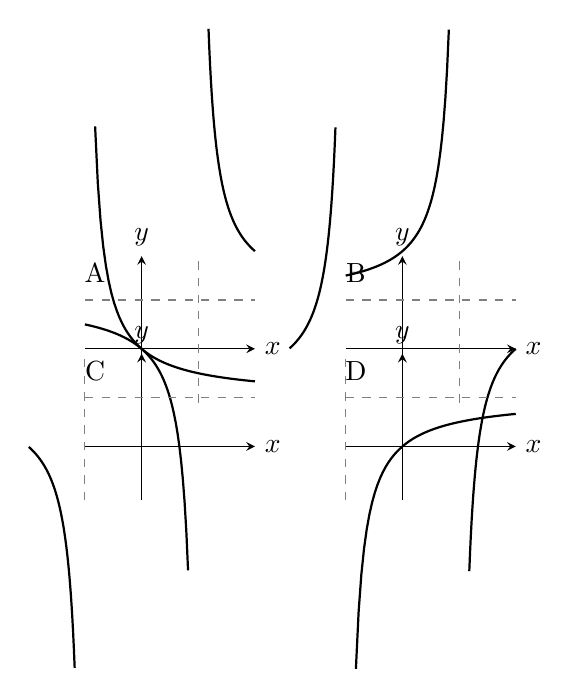
\begin{tikzpicture}[x=0.72cm,y=0.62cm,>=stealth]
  \foreach \sx/\sy/\optlabel in {0/2/A,4.6/2/B,0/0/C,4.6/0/D}
  {
    \begin{scope}[shift={(\sx,\sy)}]
      \draw[->] (-1.0,0)--(2.0,0) node[right] {$x$};
      \draw[->] (0,-1.1)--(0,1.9) node[above] {$y$};
      \node at (-0.82,1.55) {\optlabel};
    \end{scope}
  }
  % A: y=1+1/(x-1)
  \begin{scope}[shift={(0,2)}]
    \draw[dashed,gray] (1,-1.1)--(1,1.9);
    \draw[dashed,gray] (-1,1)--(2,1);
    \draw[thick,domain=-1:0.82,samples=60] plot (\x,{1+1/(\x-1)});
    \draw[thick,domain=1.18:2,samples=60] plot (\x,{1+1/(\x-1)});
  \end{scope}
  % B: y=1-1/(x-1), the correct graph
  \begin{scope}[shift={(4.6,2)}]
    \draw[dashed,gray] (1,-1.1)--(1,1.9);
    \draw[dashed,gray] (-1,1)--(2,1);
    \draw[thick,domain=-1:0.82,samples=60] plot (\x,{1-1/(\x-1)});
    \draw[thick,domain=1.18:2,samples=60] plot (\x,{1-1/(\x-1)});
  \end{scope}
  % C and D use x=-1, distinguishing the remaining distractors.
  \begin{scope}[shift={(0,0)}]
    \draw[dashed,gray] (-1,-1.1)--(-1,1.9);
    \draw[dashed,gray] (-1,1)--(2,1);
    \draw[thick,domain=-0.82:2,samples=60] plot (\x,{1+1/(\x+1)});
    \draw[thick,domain=-1.99:-1.18,samples=60] plot (\x,{1+1/(\x+1)});
  \end{scope}
  \begin{scope}[shift={(4.6,0)}]
    \draw[dashed,gray] (-1,-1.1)--(-1,1.9);
    \draw[dashed,gray] (-1,1)--(2,1);
    \draw[thick,domain=-0.82:2,samples=60] plot (\x,{1-1/(\x+1)});
    \draw[thick,domain=-1.99:-1.18,samples=60] plot (\x,{1-1/(\x+1)});
  \end{scope}
\end{tikzpicture}
\end{center}
\nopagebreak[4]
（A）　　（B）　　（C）　　（D）

\end{question}
\begin{question}
\gkti{11}从正方体的 6 个面中选取 3 个面，其中有 2 个面不相邻的选法共有\mbox{（　　）}

（A）8 种　　（B）12 种　　（C）16 种　　（D）20 种

\end{question}
\begin{question}
\gkti{12}据 2002 年 3 月 5 日九届人大五次会议《政府工作报告》：“2001 年国内生产总值达到 95933 亿元，比上年增长 $7.3\%\mbox{\fontspec{STSong}\char"3002}$”如果“十五”（2001—2005 年）期间每年的国内生产总值都按此年增长率增长，那么到“十五”末我国国内年生产总值约为\mbox{（　　）}

（A）115000 亿元　　（B）120000 亿元　　（C）127000 亿元　　（D）135000 亿元

\end{question}
\gkpart{二、填空题}

\begin{question}
\gkti{13}函数 $y=a^x$ 在 $[0,1]$ 上的最大值与最小值之和为 $3$，则 $a=$\gkblank{}。

\end{question}
\begin{question}
\gkti{14}椭圆 $5x^2+ky^2=5$ 的一个焦点是 $(0,2)$，那么 $k=$\gkblank{}。

\end{question}
\begin{question}
\gkti{15}$(x^2+1)(x-2)^7$ 展开式中 $x^3$ 的系数是\gkblank{}。

\end{question}
\begin{question}
\gkti{16}已知

\nopagebreak[4]
\[
f(x)=\frac{x^2}{1+x^2},
\]

\Needspace{5\baselineskip}
那么

\nopagebreak[4]
\[
f(1)+f(2)+f\left(\frac12\right)+f(3)+f\left(\frac13\right)+f(4)+f\left(\frac14\right)=\_\_\_\_\_\_\mbox{\fontspec{STSong}\char"3002}
\]

\end{question}
\gkpart{三、解答题}

\begin{question}
\gkti{17}已知

\nopagebreak[4]
\[
\sin^2 2\alpha+\sin2\alpha\cos\alpha-\cos2\alpha=1,\qquad
\alpha\in\left(0,\frac\pi2\right),
\]

求 $\sin\alpha\text{、}\tan\alpha$ 的值。

\Needspace{0.4\textheight}
\end{question}
\begin{question}
\gkti{18}如图，正方形 $ABCD\text{、}ABEF$ 的边长都是 $1$，而且平面 $ABCD\text{、}ABEF$ 互相垂直。点 $M$ 在 $AC$ 上移动，点 $N$ 在 $BF$ 上移动，若 $CM=BN=a$（$0<a<\sqrt2$）。
\nopagebreak[4]
\begin{center}% 2002 年全国旧课程理科第 18 题：两个互相垂直的正方形
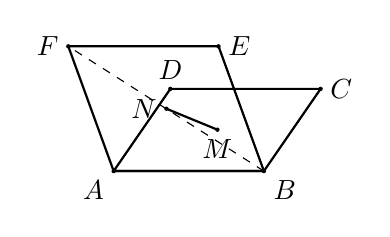
\begin{tikzpicture}[>=stealth,scale=0.72]
  \coordinate (A) at (0,0);
  \coordinate (B) at (2.65,0);
  \coordinate (C) at (3.65,1.45);
  \coordinate (D) at (1.0,1.45);
  \coordinate (E) at (1.85,2.20);
  \coordinate (F) at (-0.80,2.20);
  \coordinate (M) at (1.83,0.73);
  \coordinate (N) at (0.93,1.10);
  \draw[thick] (A)--(B)--(C)--(D)--cycle;
  \draw[thick] (A)--(B)--(E)--(F)--cycle;
  \draw[dashed] (A)--(D) (B)--(F);
  \draw[thick] (M)--(N);
  \fill (A) circle (1.1pt) node[below left] {$A$};
  \fill (B) circle (1.1pt) node[below right] {$B$};
  \fill (C) circle (1.1pt) node[right] {$C$};
  \fill (D) circle (1.1pt) node[above] {$D$};
  \fill (E) circle (1.1pt) node[right] {$E$};
  \fill (F) circle (1.1pt) node[left] {$F$};
  \fill (M) circle (1.1pt) node[below] {$M$};
  \fill (N) circle (1.1pt) node[left] {$N$};
\end{tikzpicture}
\end{center}
\nopagebreak[4]
（1） 求 $MN$ 的长；

（2） $a$ 为何值时，$MN$ 的长最小；

（3） 当 $MN$ 的长最小时，求面 $MNA$ 与面 $MNB$ 所成二面角 $\alpha$ 的大小。

\end{question}
\begin{question}
\gkti{19}设点 $P$ 到点 $(-1,0)\text{、}(1,0)$ 距离之差为 $2m$，到 $x\text{、}y$ 轴的距离之比为 $2$，求 $m$ 的取值范围。

\end{question}
\begin{question}
\gkti{20}某城市 2001 年末汽车保有量为 30 万辆，预计此后每年报废上一年末汽车保有量的 $6\%$，并且每年新增汽车数量相同。为保护城市环境，要求该城市汽车保有量不超过 60 万辆，那么每年新增汽车数量不应超过多少辆？

\end{question}
\begin{question}
\gkti{21}设 $a$ 为实数，函数

\nopagebreak[4]
\[
f(x)=x^2+|x-a|+1,\qquad x\in\mathbb R.
\]

（1） 讨论 $f(x)$ 的奇偶性；

（2） 求 $f(x)$ 的最小值。

\end{question}
\begin{question}
\gkti{22}设数列 $\{a_n\}$ 满足

\nopagebreak[4]
\[
a_{n+1}=a_n^2-na_n+1,\qquad n=1,2,3,\ldots.
\]

（1） 当 $a_1=2$ 时，求 $a_2,a_3,a_4$，并由此猜测 $a_n$ 的一个通项公式；

（2） 当 $a_1\geqslant3$ 时，证明对所有的 $n\geqslant1$，有

① $a_n\geqslant n+2$；

\Needspace{5\baselineskip}
②

\nopagebreak[4]
\[
\frac1{1+a_1}+\frac1{1+a_2}+\frac1{1+a_3}+\cdots+\frac1{1+a_n}\leqslant\frac12.
\]

\end{question}